\documentclass[a4paper,12pt]{article}

\usepackage{fancyhdr}
\usepackage{lastpage}
\usepackage{amsmath}
\usepackage{tikz}
\usepackage{amsfonts}
\usepackage{graphicx}

\pagestyle{fancy}
\lhead{Samuel Loomis}
\setlength{\headheight}{15pt}
\chead{Electromagnetism HW 4}
\rhead{\thepage\ of \pageref{LastPage}}
\lfoot{}
\cfoot{}
\rfoot{}

\begin{document}

\subsection*{Question 1}
Two semi-infinite large magnetic materials with permeability $\mu_1$\ and $\mu_2$\  meet at z = 0 plane.  Inside one of the material there is a current \textit{I} running in the y direction, at a distance d from the interface.  Calculate the magnetic field in each of the materials.

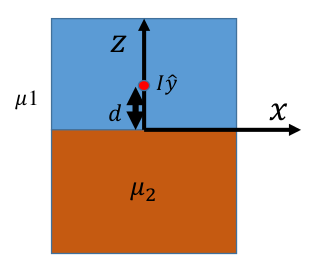
\includegraphics{Magnetic_Image.png}

The free current inside the blue material will create a bound current in the blue material, as well as inducing an `Image' current in the brown material.  At the boundary between two magenetic materials, $\frac{B_{1tang}}{\mu_1}=\frac{B_{2tang}}{\mu_2}$.  This can be achieved by replacing the brown material by a current carrying wire that would generate a magnetic field similar yet in the opposite direction as the original wire. 

 The magnetic field generated by the wire inside the blue material (not taking into account the image in brown just yet) will be easier to describe using the `$\mathbf{H}$'\ field.  the curl of \textbf{H} is equal to the free current. $\nabla \times \mathbf{H}=\mathbf{J_f}$

\end{document}


